%% ============================================================================
%%  Ambient WiFi as a Radar Replacement for Automotive SLAM
%%  A physics-based (Sionna RT) feasibility study.
%%
%%  Target: Q1 journal (e.g. IEEE IoT-J / IEEE Sensors J. / IEEE T-ITS).
%%  Build:  latexmk -pdf main.tex   (or upload the paper/ folder to Overleaf)
%%
%%  STATUS: skeleton. Sub-7 GHz localization + sensing + mapping sections are
%%  written from the released results (docs/results-v1.md, v0.4.0). The 60 GHz
%%  extension (Sec. VII) and any real-CSI validation are PENDING and are marked
%%  with %% TODO. Numbers tagged %% CHECK should be re-read from the artifacts
%%  before submission.
%% ============================================================================
\documentclass[journal]{IEEEtran}

\usepackage{amsmath,amssymb}
\usepackage{graphicx}
\usepackage{booktabs}
\usepackage{siunitx}
\usepackage{url}
\usepackage[hidelinks]{hyperref}
\graphicspath{{../docs/assets/}}

\begin{document}

\title{Ambient WiFi as a Radar Replacement for Automotive SLAM:\\
A Physics-Based Feasibility Study}

\author{Mulham Fetna%
\thanks{M. Fetna is an independent researcher (robotics/mechatronics).
E-mail: contact@mulhamfetna.com. ORCID: 0009-0006-4432-798X.}%
\thanks{Code, configurations and results are openly available and citable:
GitHub \url{https://github.com/mulhamfetna/wifi-radar-slam};
Zenodo concept DOI \texttt{10.5281/zenodo.21247288}.}}

\maketitle

\begin{abstract}
Automotive radar is a costly, dedicated sensor, while WiFi transceivers are
ubiquitous and, under the integrated sensing and communication (ISAC) paradigm,
increasingly dual-purpose. We ask whether \emph{ambient} sub-\SI{7}{GHz}
WiFi---received on a single moving-vehicle antenna and processed with commodity
channel-state information (CSI)---can serve in place of radar as the perception
front-end of a SLAM pipeline. Using physics-based ray tracing (Sionna RT), we
build an end-to-end pipeline: ray-traced multipath channel $\rightarrow$
super-resolution (MUSIC) delay/angle estimation $\rightarrow$ bistatic reflector
triangulation $\rightarrow$ Rao--Blackwellized particle-filter SLAM, and evaluate
it with trajectory (ATE/RPE) and map (Chamfer, occupancy IoU, directional
accuracy/completeness) metrics. We find that ambient WiFi \emph{localizes} the
vehicle to centimetre level with a clean operating envelope that follows the
$\Delta R = c/2B$ resolution law, and that a joint two-dimensional (delay--angle)
MUSIC front-end lifts \emph{realistic} commodity-CSI localization to
oracle-sensing quality in sparse-multipath scenes. In contrast, \emph{mapping}
separates into two tiers: with clean single-bounce (oracle) sensing the back-end
reconstructs reflecting surfaces to \SIrange{25}{30}{cm}, whereas realistic
sensing is bounded to \SIrange{4}{5}{m} by a systematic delay-estimation bias in
dense multipath---not by bandwidth or array aperture. These results delineate
precisely what passive sub-\SI{7}{GHz} WiFi can and cannot do for automotive
SLAM, and motivate a \SI{60}{GHz} extension as the physical remedy for the
mapping limitation.
\end{abstract}

\begin{IEEEkeywords}
WiFi sensing, passive WiFi radar, channel state information, SLAM, integrated
sensing and communication, automotive perception, multipath-based SLAM, Sionna RT.
\end{IEEEkeywords}

% ============================================================================
\section{Introduction}
% ============================================================================
\IEEEPARstart{A}{utomotive} perception relies heavily on radar for its robustness
to weather and lighting, but radar is a dedicated, cost- and power-bearing sensor.
In parallel, WiFi radios are ubiquitous---in vehicles, roadside units and the
built environment---and the emerging ISAC paradigm and the IEEE~802.11bf sensing
amendment are turning communication hardware into opportunistic sensors
\cite{overview2024ieee80211bf,liu2022isac,zhang2021jcassurvey}. This raises a
concrete question for autonomous systems: \emph{can ambient WiFi, received on a
moving vehicle, replace radar as the perception input to SLAM?}

\textbf{The gap.} A two-round, adversarially fact-checked survey (summarized in
Sec.~\ref{sec:related}) exposes a clean and defensible gap. Passive WiFi radar and
CSI-based sensing are mature but almost exclusively \emph{indoor, static and
infrastructure-fixed}
\cite{chetty2012ttwifi,yildirim2021superres,li2021standalone,yan2024personinwifi3d};
the one demonstrated \emph{moving-platform} passive radar uses a 5G downlink---not
WiFi---as its illuminator \cite{maksymiuk2024movingpr}; and joint communication
and SLAM is explicitly ``in its infancy'' \cite{gounis2026slamcomms}. No prior work
occupies the intersection of an \emph{on-vehicle, mobile, outdoor, WiFi-band}
sensing system feeding a SLAM pipeline.

\textbf{The physical fork.} Range resolution is bandwidth-limited,
$\Delta R = c/2B$: commodity sub-\SI{7}{GHz} WiFi resolves only
\SI{3.75}{m} at \SI{40}{MHz} and \SI{0.94}{m} at \SI{160}{MHz}, whereas radar-grade
resolution (\(\sim\)\SI{8.5}{cm}) requires \SI{60}{GHz} mmWave (IEEE~802.11ad DMG)
\cite{kumari2018adradar,overview2024ieee80211bf}. A WiFi-for-SLAM design must
therefore either (i) stay sub-\SI{7}{GHz} and extract coarse geometry from
multipath, or (ii) move to \SI{60}{GHz} for fine range. \emph{This paper takes the
sub-\SI{7}{GHz} path and characterizes it honestly and end-to-end}, isolating what
is achievable now from what needs the mmWave extension.

\textbf{Contributions.}
\begin{itemize}
\item An open, reproducible, physics-based (Sionna RT ray-traced) end-to-end
pipeline for on-vehicle ambient-WiFi SLAM, spanning channel simulation,
super-resolution sensing, bistatic mapping and particle-filter SLAM.
\item A demonstration that ambient sub-\SI{7}{GHz} WiFi \emph{localizes} a moving
vehicle to centimetre level, with an operating envelope (bandwidth, SNR, access
points, speed) that quantitatively follows the $\Delta R=c/2B$ law.
\item A \emph{joint two-dimensional (delay--angle) MUSIC} front-end whose intrinsic
association lifts realistic commodity-CSI localization to oracle-sensing quality
in sparse multipath.
\item A two-tier characterization of \emph{mapping}: an oracle upper bound
(\SIrange{25}{30}{cm}) and a realistic bound (\SIrange{4}{5}{m}), with the residual
gap pinned to a delay-estimation bias in dense multipath rather than to bandwidth
or aperture---clarifying exactly what further sensing advances mapping requires.
\end{itemize}

% ============================================================================
\section{Related Work}\label{sec:related}
% ============================================================================
\subsection{Passive WiFi Radar}
Ambient WiFi access points act as illuminators of opportunity for bistatic passive
radar. Chetty \emph{et al.} first demonstrated through-wall detection of moving
personnel, extracting both range and Doppler \cite{chetty2012ttwifi}. Because WiFi
bursts have short integration time and low bandwidth, standard Fourier processing
is inadequate, motivating super-resolution (ESPRIT/MUSIC) methods
\cite{yildirim2021superres}; passive radar has been shown against unmodified
stand-alone access points \cite{li2021standalone}, and phase-robust CSI-power
processing achieves sub-metre indoor tracking \cite{wang2025csipower}. All of this
work is indoor and static---the point of departure for a mobile outdoor system.

\subsection{WiFi CSI Sensing and 3D Reconstruction}
WiFi-band signals reflect off bodies and penetrate walls; learning-based methods
reconstruct dense structure---2D/3D human pose
\cite{zhao2018rfpose,zhao2018rfpose3d,yan2024personinwifi3d,wang2019personinwifi},
depth \cite{widepth2025}, and even latent-diffusion imagery \cite{latentcsi2025}.
These systems prove dense WiFi ``imaging'' is possible, but every one is a
few-metre \emph{fixed indoor} zone with poor cross-environment generalization
\cite{yan2024personinwifi3d}---which both motivates and bounds the present work.
We are careful to distinguish purpose-built WiFi-band FMCW radios
\cite{zhao2018rfpose} from decoded commodity 802.11 CSI \cite{wang2019personinwifi}.

\subsection{RF- and Multipath-based SLAM}
The SLAM back-end we require already exists. Channel-SLAM treats each multipath
component as a line-of-sight signal from a \emph{virtual transmitter}, jointly
estimating landmark and receiver states with no prior map
\cite{gentner2016channelslam,ulmschneider2017multipath}; modern multipath-based
SLAM extends this with cooperation, map fusion and belief propagation, including
real mmWave-MIMO measurements
\cite{leitinger2024mpslamcoop,li2024bpmpslam}. We reuse this virtual-transmitter /
bistatic-reflector landmark model and test its robustness to a fast-moving receiver.

\subsection{ISAC, IEEE 802.11bf and mmWave WiFi}
ISAC formalizes the shared-hardware sensing/communication tradeoff
\cite{liu2022isac,xiong2023scfundamental,zhang2021jcassurvey}, and IEEE~802.11bf
standardizes the sensing measurement plumbing while leaving algorithms to vendors
\cite{overview2024ieee80211bf}. Crucially for our design fork, the 802.11ad
\SI{60}{GHz} waveform has been reused as a radar with $<$\SI{0.1}{m} range
resolution and V2I imaging, albeit in theory/simulation
\cite{kumari2018adradar,han2022adimaging}. This frames our sub-\SI{7}{GHz}-now,
\SI{60}{GHz}-next roadmap.

% ============================================================================
\section{System Model and Method}\label{sec:method}
% ============================================================================
\subsection{Scenario and Bistatic Geometry}
A vehicle carrying a single receive antenna array drives through an outdoor scene
illuminated by $N_\mathrm{AP}$ ambient WiFi access points at known positions.
Each specular multipath component follows an access point $\rightarrow$ reflector
$\rightarrow$ vehicle path, so the measured path length
$\rho = \lVert\mathbf{p}_\mathrm{AP}-\mathbf{r}\rVert +
\lVert\mathbf{r}-\mathbf{p}_\mathrm{veh}\rVert$ places the reflector $\mathbf{r}$ on
an ellipse with foci at the access point and the vehicle. Given the arrival azimuth
$\phi$ (the bearing from the vehicle to $\mathbf{r}$), the reflector range $s$ along
$\hat{\mathbf u}(\phi)$ solves
\begin{equation}
s = \frac{\rho^2 - d_\mathrm{AP}^2}{2\big(\rho - \mathbf{d}_\mathrm{AP}\!\cdot\!\hat{\mathbf u}(\phi)\big)},
\qquad \mathbf{d}_\mathrm{AP} = \mathbf{p}_\mathrm{AP}-\mathbf{p}_\mathrm{veh},
\label{eq:bistatic}
\end{equation}
with $d_\mathrm{AP}=\lVert\mathbf{d}_\mathrm{AP}\rVert$; the direct path
($s\!\le\!0$) and physically implausible solves are rejected.

\subsection{Ray-Traced Channel Model}
Channels are generated with Sionna RT~2.0 (Mitsuba/Dr.Jit), which ray-traces the
scene (buildings, vehicles) to produce per-path delays, angles, interaction types
and the frequency-domain channel (CFR) across $N_\mathrm{sc}$ OFDM subcarriers and
$N_\mathrm{rx}$ antennas, per vehicle pose along the trajectory. Additive white
Gaussian noise is applied at a configured SNR.

\subsection{Sensing Front-End}
We compare two sensing tiers. The \emph{oracle} front-end reads Sionna's true
single-scatter path parameters (delay, azimuth), isolating the mapping/SLAM
geometry from estimation error. The \emph{realistic} front-end estimates parameters
from the noisy CSI with MUSIC. For delays we use the antennas as snapshots over a
physically-bounded delay grid; for azimuth we use the subcarriers as snapshots. A
key refinement is \emph{joint 2-D (delay--angle) MUSIC} with 2-D spatial smoothing
(SVD subspace; delay grid bounded to the unambiguous $1/\Delta f$ range), which
recovers each path's delay \emph{and} angle together, so their association is
intrinsic rather than paired by sorted index. Array-relative electrical angles are
mapped to world azimuth by $\sin\beta=-\sin\theta$ for the vehicle's lateral ULA.

\subsection{SLAM Back-End and Metrics}
A Rao--Blackwellized particle filter propagates the vehicle pose from odometry and
weights particles by the bistatic consistency \eqref{eq:bistatic} of each
detection; triangulated reflectors are accumulated and consensus-filtered into a
landmark map. We report trajectory error (ATE, RPE) and, for the map, symmetric
Chamfer distance, occupancy IoU, and \emph{directional} accuracy (estimate
$\rightarrow$ ground truth) and completeness (ground truth $\rightarrow$ estimate),
since a passive-WiFi map illuminates only a subset of surfaces. Ground truth for the
map is the facade footprint of each scene object.

% ============================================================================
\section{Experimental Setup}\label{sec:setup}
% ============================================================================
Two scene families are used. A \emph{street canyon} (Sionna's
\texttt{simple\_street\_canyon\_with\_cars}) provides a realistic, dense-multipath
outdoor environment; a \emph{controlled reflective} scene (a scaled metal wall)
provides a geometry in which clean single-bounce returns are guaranteed, isolating
sensing from illumination effects. Unless stated otherwise: carrier
\SI{5.2}{GHz}, \SI{40}{MHz} bandwidth, $N_\mathrm{sc}=64$, $N_\mathrm{rx}=4$
(half-wavelength ULA), \num{3} access points, \SI{20}{dB} SNR, \SI{5}{m/s} straight
trajectory. Simulations run CPU-only (Sionna RT LLVM backend) on a 32-thread
workstation; each Phase-A run completes in tens of seconds.
%% CHECK: confirm exact nominal config against configs/nominal.yaml before submission.

\begin{figure}[t]
\centering
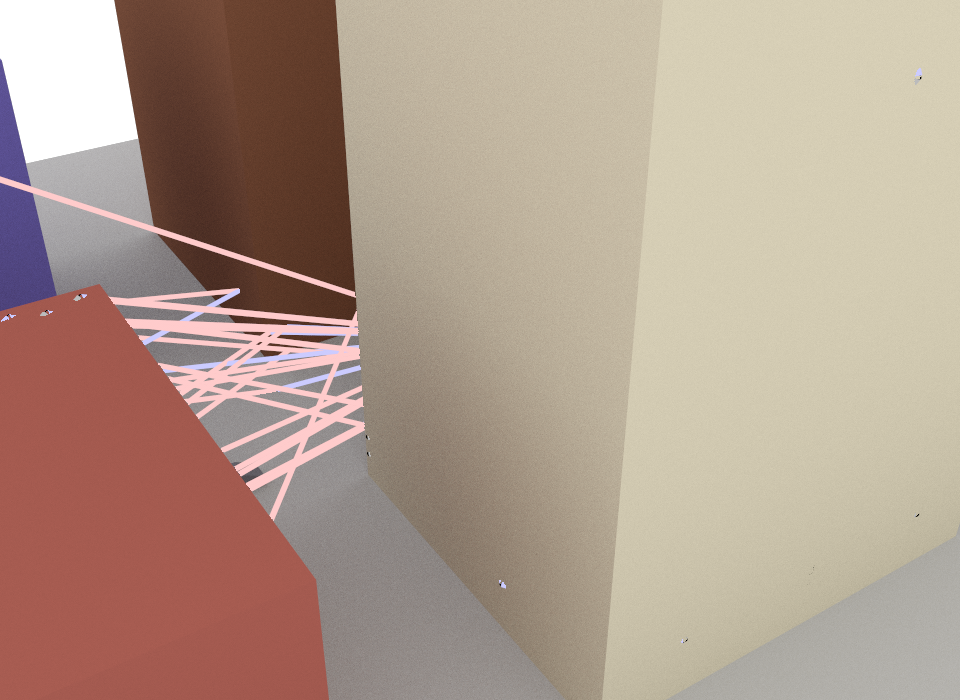
\includegraphics[width=0.95\columnwidth]{scene_paths.png}
\caption{Ray-traced street-canyon scene with the ambient-WiFi multipath rays from
an access point to the vehicle antenna (Sionna RT render).}
\label{fig:scene}
\end{figure}

% ============================================================================
\section{Results}\label{sec:results}
% ============================================================================
\subsection{Localization Operating Envelope}
Ambient WiFi localizes the vehicle to centimetre level. Table~\ref{tab:envelope}
sweeps the four principal parameters. Bandwidth shows the expected monotonic
$\sim$20$\times$ ATE improvement from \SI{20}{MHz} to \SI{160}{MHz}, tracking the
$\Delta R=c/2B$ law end-to-end; SNR degrades gracefully to sub-decimetre by
\SI{30}{dB}; more access points and higher speeds are generally beneficial.

\begin{table}[t]
\caption{Localization operating envelope: absolute trajectory error (ATE, m),
one parameter swept at a time about the nominal point.}
\label{tab:envelope}
\centering
\small
\begin{tabular}{@{}llll@{}}
\toprule
\multicolumn{2}{c}{Bandwidth} & \multicolumn{2}{c}{SNR}\\
\SI{20}{MHz} & 0.78 & \SI{0}{dB} & 2.02\\
\SI{40}{MHz} & 0.093 & \SI{10}{dB} & 1.86\\
\SI{80}{MHz} & 0.058 & \SI{20}{dB} & 1.01\\
\SI{160}{MHz} & 0.038 & \SI{30}{dB} & 0.076\\
\midrule
\multicolumn{2}{c}{\# Access points} & \multicolumn{2}{c}{Speed}\\
1 & 0.084 & \SI{1}{m/s} & 2.13\\
2 & 1.97 & \SI{5}{m/s} & 0.032\\
3 & 0.075 & \SI{10}{m/s} & 0.047\\
4 & 0.041 & \SI{15}{m/s} & 0.010\\
\bottomrule
\end{tabular}
\end{table}
%% CHECK: numbers from docs/results-v1.md Phase B; regenerate table from results if configs change.

\subsection{Realistic Sensing: Joint Delay--Angle MUSIC}
Separate 1-D delay and 1-D angle estimates paired by sorted index mis-associate in
multipath and scatter phantom reflectors. Joint 2-D MUSIC removes this by estimating
each path's delay and angle together. In the controlled scene at \SI{160}{MHz},
realistic ATE improves from \SI{0.73}{m} (sorted) to \SI{0.027}{m} (joint),
matching the \SI{0.045}{m} oracle bound---i.e.\ \emph{realistic commodity-CSI
localization becomes oracle-quality} in sparse multipath. The benefit is
scene-dependent: in the dense street canyon (\(\sim\)19 paths, 4 antennas) the paths
cannot be resolved and joint estimation does not help, so it is retained as an
opt-in front-end.

\subsection{Mapping: Oracle vs.\ Realistic}
Table~\ref{tab:map} contrasts the two sensing tiers. With oracle sensing the map
reconstructs reflecting surfaces to \SIrange{25}{30}{cm}
(Fig.~\ref{fig:maps}, left); the same geometry under realistic MUSIC sensing is
bounded to \SIrange{4}{5}{m}. Critically, this residual persists even in the
front/back-unambiguous controlled scene and even under wider bandwidth and joint
estimation, so it is a \emph{delay-estimation bias in dense multipath}, not an
association or aperture problem. Passive-WiFi mapping therefore requires further
sensing advances (bounce discrimination, wider bandwidth) beyond super-resolution
on a single commodity link.

\begin{table}[t]
\caption{Mapping accuracy: oracle vs.\ realistic sensing.}
\label{tab:map}
\centering
\small
\begin{tabular}{@{}lccc@{}}
\toprule
Scene / sensing & accuracy (m) & Chamfer (m) & IoU\\
\midrule
Controlled wall, oracle & 0.25 & 0.51 & 0.79\\
Street canyon, oracle & 0.30 & 12.3\,$^\dagger$ & 0.08\\
Controlled wall, realistic (joint) & 4.8 & 4.1 & 0.0\\
\bottomrule
\end{tabular}
\\[2pt]
\raggedright\footnotesize $^\dagger$ symmetric Chamfer inflated by partial
coverage; a single WiFi pass illuminates only street-facing facades.
\end{table}
%% CHECK: numbers from docs/results-v1.md ("Mapping demonstration" + "Realistic sensing").

\begin{figure}[t]
\centering
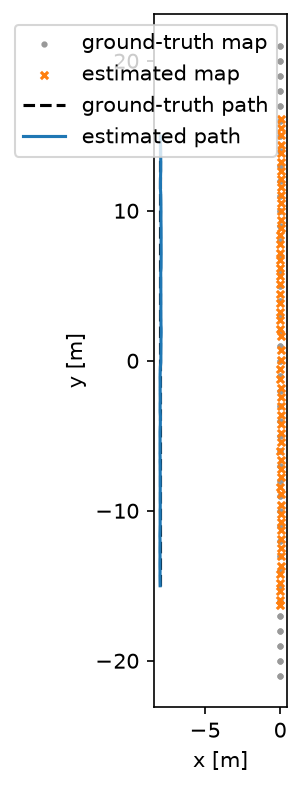
\includegraphics[width=0.48\columnwidth]{controlled_map.png}\hfill
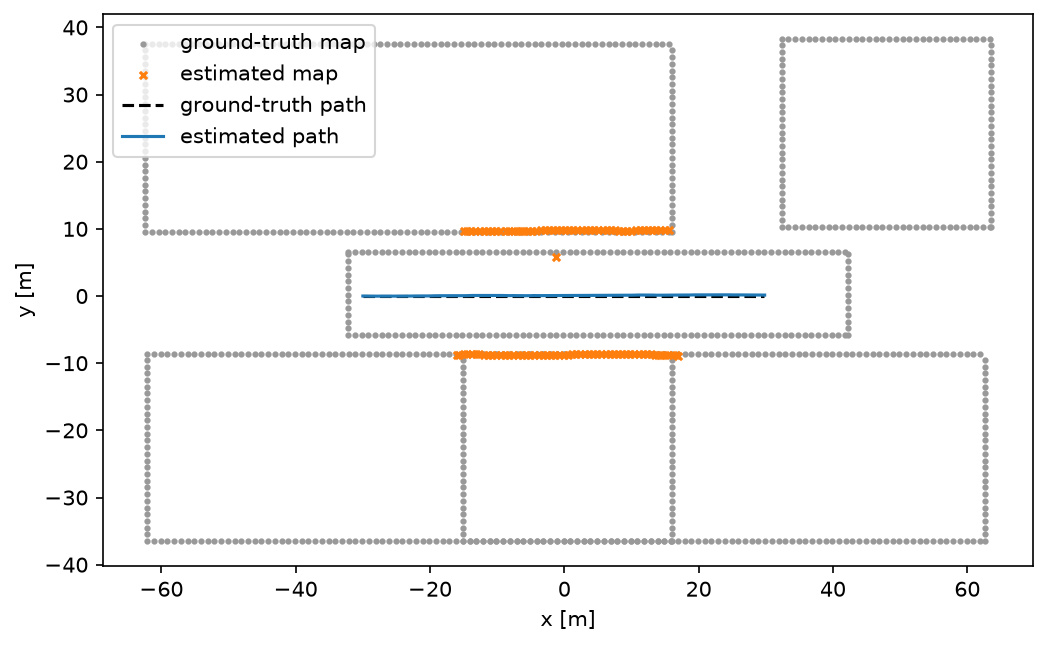
\includegraphics[width=0.48\columnwidth]{street_metal_map.png}
\caption{Oracle maps. Left: controlled wall---estimated reflectors (orange) trace
the wall to \(\sim\)\SI{0.25}{m}. Right: reflective street canyon---reflectors
trace the two illuminated street-facing facades; distant/outer surfaces are
uncovered (coverage, not accuracy, limited).}
\label{fig:maps}
\end{figure}

% ============================================================================
\section{Discussion}
% ============================================================================
The results delineate a clear boundary. \emph{Localization} from ambient
sub-\SI{7}{GHz} WiFi is practical today: centimetre-level and, with joint
estimation, oracle-quality from realistic CSI in favourable geometry. \emph{Mapping}
is fundamentally harder: the low bandwidth blends dense multipath, biasing delay
estimates and flooring realistic map accuracy at a few metres. This is the physical
signature of the $\Delta R=c/2B$ ceiling, and it is precisely what a wider-band
\SI{60}{GHz} front-end would relieve. Limitations of this study are its
simulation-only scope and the single-array receiver; both are addressed in the
roadmap below.

% ============================================================================
\section{The 60\,GHz Extension (Ongoing)}\label{sec:60ghz}
% ============================================================================
%% TODO: run and write. The mapping limitation above is a bandwidth problem; the
%% 60 GHz (802.11ad DMG, ~1.76 GHz) waveform gives DR ~ 8.5 cm and should resolve
%% the dense multipath that biases sub-7 GHz delay estimation, enabling realistic
%% mapping. Plan: (i) wide-band Sionna sim at 60 GHz with Golay-preamble-style
%% sensing; (ii) re-run the same pipeline/metrics; (iii) test whether cm-resolution
%% removes the ~5 m realistic map bias. Compare against Kumari et al. \cite{kumari2018adradar}.
The mapping limitation identified above is, by construction, a bandwidth problem.
A \SI{60}{GHz} (IEEE~802.11ad DMG) front-end offers \(\sim\)\SI{1.76}{GHz} of
bandwidth ($\Delta R\approx\SI{8.5}{cm}$) and is the natural remedy. This extension
is in progress and will be reported in a subsequent revision.

% ============================================================================
\section{Conclusion}
% ============================================================================
We presented an open, physics-based feasibility study of ambient sub-\SI{7}{GHz}
WiFi as a radar replacement for automotive SLAM. Ambient WiFi localizes a moving
vehicle to centimetre level---and to oracle-sensing quality from realistic CSI via
joint delay--angle MUSIC in sparse multipath---while mapping separates into an
oracle upper bound (\SIrange{25}{30}{cm}) and a realistic bound
(\SIrange{4}{5}{m}) set by delay-estimation bias in dense multipath. The study thus
maps the boundary of the achievable for passive sub-\SI{7}{GHz} WiFi perception and
motivates a \SI{60}{GHz} extension to close the mapping gap.

\section*{Reproducibility}
All code, configurations, scenes and result artifacts are openly available:
GitHub \url{https://github.com/mulhamfetna/wifi-radar-slam}; archived on Zenodo
(concept DOI \texttt{10.5281/zenodo.21247288}).

\bibliographystyle{IEEEtran}
\bibliography{refs}

\end{document}
